%%%%%%%%%%%%%%%%%%%%%%%%%%%%%%%%%%%%%%%%%
% Developer CV
% LaTeX Template
% Version 1.0 (28/1/19)
%
% This template originates from:
% http://www.LaTeXTemplates.com
%
% Authors:
% Jan Vorisek (jan@vorisek.me)
% Based on a template by Jan Küster (info@jankuester.com)
% Modified for LaTeX Templates by Vel (vel@LaTeXTemplates.com)
%
% License:
% The MIT License (see included LICENSE file)
%
%%%%%%%%%%%%%%%%%%%%%%%%%%%%%%%%%%%%%%%%%

%----------------------------------------------------------------------------------------
%	PACKAGES AND OTHER DOCUMENT CONFIGURATIONS
%----------------------------------------------------------------------------------------

\documentclass[9pt]{developercv} % Default font size, values from 8-12pt are recommended
\usepackage{graphicx}

%----------------------------------------------------------------------------------------

\begin{document}

%----------------------------------------------------------------------------------------
%	TITLE AND CONTACT INFORMATION
%----------------------------------------------------------------------------------------

\begin{minipage}[t]{0.55\textwidth} % 45% of the page width for name
	\vspace{-\baselineskip} % Required for vertically aligning minipages
	
	% If your name is very short, use just one of the lines below
	% If your name is very long, reduce the font size or make the minipage wider and reduce the others proportionately
	\colorbox{black}{{\HUGE\textcolor{white}{\textbf{\MakeUppercase{Maksim}}}}} % First name
	
	\colorbox{black}{{\HUGE\textcolor{white}{\textbf{\MakeUppercase{Bronnikov}}}}} % Last name
	
	\vspace{7pt}
	
	{\huge C++ developer} % Career or current job title
	
\end{minipage}
\begin{minipage}[t]{0.45\textwidth} % 45% of the page width for name
	\vspace{-\baselineskip} % Required for vertically aligning minipages
	
	\hspace*{3.9cm}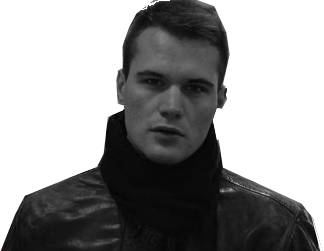
\includegraphics[scale = 0.39]{max.png}\\
	
\end{minipage}

\vspace{0.2cm}

\begin{minipage}[t]{0.275\textwidth} % 27.5% of the page width for the first row of icons
	\vspace{-\baselineskip} % Required for vertically aligning minipages
	
	% The first parameter is the FontAwesome icon name, the second is the box size and the third is the text
	% Other icons can be found by referring to fontawesome.pdf (supplied with the template) and using the word after \fa in the command for the icon you want
	\icon{MapMarker}{12}{Podgorica, Montenegro}\\
	\icon{Phone}{12}{+7 953 335 68 73}\\
	\icon{At}{12}{\href{mailto:max120199@gmail.com}{max120199@gmail.com}}\\	
\end{minipage}
\begin{minipage}[t]{0.275\textwidth} % 27.5% of the page width for the second row of icons
	\vspace{-\baselineskip} % Required for vertically aligning minipages
	\icon{Vk}{12}{\href{https://vk.com/mbronnikov}{vk.com/mbronnikov}}\\
	\icon{Github}{12}{\href{https://github.com/m-bronnikov}{github.com/m-bronnikov}}\\
	\icon{PaperPlane}{12}{\href{https://t.me/decrement}{@decrement}}\\
	% The first parameter is the FontAwesome icon name, the second is the box size and the third is the text
	% Other icons can be found by referring to fontawesome.pdf (supplied with the template) and using the word after \fa in the command for the icon you want
	
\end{minipage}

\vspace{0.1cm}

%----------------------------------------------------------------------------------------
%	INTRODUCTION, SKILLS AND TECHNOLOGIES
%----------------------------------------------------------------------------------------

\cvsect{About me}

\begin{minipage}[t]{0.55\textwidth} % 40% of the page width for the introduction text
	\vspace{-\baselineskip} % Required for vertically aligning minipages
I create efficient programs with C++ and search non-standard solutions to any tasks. While studying in "Applied mathematics and computer science", I received a good mathematical education, which helps to me in my work. I apply on practice knowledge of compilers and neural networks for developing elegant and beautiful optimized code. Trying to find myself in site development has rewarded me with an understanding of the main business processes and the importance of getting the job done on time. I am sure that my focus on results and desire to create can help me and my team achieve success in tasks of any complexity. 

\end{minipage}
\hfill % Whitespace between
\begin{minipage}[t]{0.40\textwidth} % 50% of the page for the skills bar chart
	\vspace{-\baselineskip} % Required for vertically aligning minipages
	\begin{barchart}{5.5}
		\baritem{C++/C}{100}
		\baritem{Python}{60}
		\baritem{ASM x86}{20}
		\baritem{Bash}{40}
	\end{barchart}
	% \vspace{0.01cm}
	\begin{center}
    \bubbles{2/Numpy, 3/STL, 2/GTest, 1/Tensorflow, 3/Git}
    \end{center}
\end{minipage}

\vspace{0.05cm}

%----------------------------------------------------------------------------------------
%	EXPERIENCE
%----------------------------------------------------------------------------------------

% TODO Add more info
\cvsect{Experience}
\begin{entrylist}
	\entry
		{2020}
		{Web Development}
		{}
		{I developed any websites, including online stores and vcard sites.\\
		\texttt{Python}\slashsep\texttt{HTML/CSS}\slashsep\texttt{Django}}
	\entry
		{2020}
		{C++ Developer}
		{CSoft}
		{Development of NanoCAD modules.  \\
		\texttt{C++}\slashsep\texttt{ObjectARX}}
	\entry
		{2020 - 2022}
		{NPU Compiler and Runtime developer}
		{Samsung Research}
		{Working on Samsung ONE neural framework and compiler for NPU.  \\
		\texttt{C++}\slashsep\texttt{Python}\slashsep\texttt{Neural Networks}\slashsep\texttt{NPU}}
	\entry
		{2022 - Present}
		{Engine developer}
		{Saber Interactive}
		{Development of internal 3D-engine for modern AAA-projects.  \\
		\texttt{C++}\slashsep\texttt{Game Dev}\slashsep\texttt{Data structures}}
		
\end{entrylist}

\vspace{0.05cm}

%----------------------------------------------------------------------------------------
%	EDUCATION
%----------------------------------------------------------------------------------------

\cvsect{Education}

\begin{entrylist}
	\entry
		{2017 -- 2021}
		{Bachelor’s Degree}
		{Moscow Aviation Institute}
		{Applied Mathematics and Computer Science}
	\entry
		{2019}
		{Course}
		{Mail.ru Group}
		{Machine Learning in MAI}
	\entry
		{2020}
		{Course}
		{Mail.Ru Group, MIPT}
		{Python for Data analysis}
	\entry
		{2021}
		{Course}
		{École Polytechnique Fédérale de Lausanne}
		{Digital Signal Processing: Basic Concepts and Algorithms}
\end{entrylist}

\vspace{0.05cm}
%----------------------------------------------------------------------------------------
%	ADDITIONAL INFORMATION
%----------------------------------------------------------------------------------------

\begin{minipage}[t]{0.2\textwidth}
	\vspace{-\baselineskip} % Required for vertically aligning minipages

	\cvsect{Languages}
	
	\textbf{Russian} - native\\
	\textbf{English} - B2 level\\

\end{minipage}
\hfill
\begin{minipage}[t]{0.40\textwidth}
	\vspace{-\baselineskip} % Required for vertically aligning minipages
	
	\cvsect{Hobbies}
	
	I'm interested in Olympiad programming, swimming and basketball.
\end{minipage}
\hfill
\begin{minipage}[t]{0.3\textwidth}
	\vspace{-\baselineskip} % Required for vertically aligning minipages
	
	\cvsect{Ready to work}
	
	I am ready to full time work, ready for remote work and relocation.
	
\end{minipage}

%----------------------------------------------------------------------------------------

\end{document}
